\documentclass[conf]{new-aiaa}
%\documentclass[journal]{new-aiaa} for journal papers

% Package Imports
\usepackage{csvsimple}
\usepackage{graphicx}
\usepackage{amsmath, amssymb}
\usepackage{siunitx}
\usepackage{listings}
\usepackage{xcolor}
\usepackage{booktabs}
\usepackage{float}
\usepackage[utf8]{inputenc}
\usepackage{listings}
\usepackage{float}
\usepackage{graphicx}
\usepackage{amsmath}
\usepackage[version=4]{mhchem}
\usepackage{siunitx}
\usepackage{longtable,tabularx}
\setlength\LTleft{0pt} 

% Title & Author
\title{Full Model Airplane Aerodynamic Force and Moment Measurements}
\author{Parham Khodadi\footnote{Aerospace Engineering student, San Diego State University}}
\affil{A E 303, Section 3, with Dr. Xiaofeng Liu}

\lstdefinestyle{pythonstyle}{
    language=Python,
    basicstyle=\ttfamily\footnotesize,
    keywordstyle=\color{blue},
    commentstyle=\color{gray},
    stringstyle=\color{orange},
    breaklines=true,
    breakatwhitespace=true,
    tabsize=4,
    frame=single,
    numbers=left,
    numberstyle=\tiny\color{gray}
}

\begin{document}

\maketitle

\begin{abstract}
This experiment evaluated the aerodynamic performance of a full aircraft model (Douglas DC-6B) in SDSU’s low-speed wind tunnel. Forces and moments were measured for various angles of attack and sideslip, with and without the tail installed. A two-level tare correction was used to isolate aerodynamic loads. 

Key results include a lift curve slope of \( \frac{dC_L}{d\alpha} = 0.0634 \), a stall at \( \alpha = 8^\circ \) with \( C_{L,\text{max}} = 0.6549 \), and a maximum lift-to-drag ratio of 16.2. Stability analysis showed tail-on configurations were stable in pitch and yaw, while tail-off cases exhibited instability. The drag polar fit yielded \( C_{D_0} = -0.0100 \) and \( e = 0.0961 \), possibly due to measurement noise. 

The experiment reinforced aerodynamic theory and highlighted practical challenges such as alignment sensitivity, RMSD noise, and tare subtraction accuracy.

\end{abstract}


\section{Nomenclature}
{\renewcommand\arraystretch{1.0}
\noindent\begin{longtable*}{@{}l @{\quad=\quad} l@{}}
\(\alpha\) & Angle of Attack (deg) \\
\(\beta\) & Sideslip Angle (deg) \\
\(C_L\) & Lift Coefficient (–) \\
\(C_D\) & Drag Coefficient (–) \\
\(C_M\) & Pitching Moment Coefficient (–) \\
\(C_N\) & Yawing Moment Coefficient (–) \\
\(F_x\) & Streamwise Force (lbs) \\
\(F_y\) & Side Force (lbs) \\
\(F_z\) & Vertical Force (lbs) \\
\(M_x\) & Rolling Moment (lb-in) \\
\(M_y\) & Pitching Moment (lb-in) \\
\(M_z\) & Yawing Moment (lb-in) \\
\(q\) & Dynamic Pressure (psi) \\
\(S\) & Wing Planform Area (in\(^2\)) \\
\(c\) & Mean Aerodynamic Chord (in) \\
\(b\) & Wing Span (in) \\
\(AR\) & Aspect Ratio (\(b^2/S\)) (–) \\
\(K\) & Induced Drag Factor (–) \\
\(C_{D,0}\) & Zero-Lift Drag Coefficient (–) \\
\(e\) & Oswald Efficiency Factor (–) \\
\(\left(\frac{C_L}{C_D}\right)_{\max}\) & Maximum Lift-to-Drag Ratio (–) \\
RMSD & Root Mean Square Deviation (units vary) \\
\(T_{\text{amb}}\) & Ambient Temperature (°F) \\
\(P_{\text{amb}}\) & Ambient Pressure (psi) \\
\end{longtable*}}


\section{Introduction}

Understanding the aerodynamic behavior of a full aircraft model is essential for evaluating flight performance, stability, and control. This experiment aims to measure and analyze the lift, drag, pitching moment, and yawing moment of a model aircraft—specifically the \textit{Douglas DC-6B}—using a subsonic wind tunnel and a six-component strain-gauge force balance system. The experiment introduces real-world complexities such as tare corrections, support interference, and ambient condition monitoring, providing hands-on reinforcement of theoretical concepts introduced in AE 301 and AE 303.

Testing is performed in the San Diego State University Low-Speed Wind Tunnel, where the model is subjected to various angles of attack (\(\alpha\)) and sideslip angles (\(\beta\)) in both tail-on and tail-off configurations. The results allow for the determination of key aerodynamic parameters such as the lift curve slope, zero-lift angle of attack, maximum lift coefficient, drag polar fit, Oswald efficiency factor, and longitudinal/directional stability slopes.

The methodology includes rigorous tare subtraction, coefficient derivation, and MATLAB-based data processing. This lab supports conceptual understanding of stability criteria and efficiency metrics relevant to both academic studies and applied aerospace design. The experiment follows standard wind tunnel protocols, and the significance of each variable is further elaborated in the Nomenclature section that follows.

\section{Theory}

The aerodynamic behavior of an aircraft can be described using nondimensional coefficients derived from measured forces and moments. These coefficients are defined as:

\begin{align}
    C_L &= \frac{F_z}{qS} &\text{(Lift coefficient)} \\
    C_D &= \frac{F_x}{qS} &\text{(Drag coefficient)} \\
    C_M &= \frac{M_y}{qSc} &\text{(Pitching moment coefficient)} \\
    C_N &= \frac{M_z}{qSb} &\text{(Yawing moment coefficient)}
\end{align}

where \( q \) is the dynamic pressure, \( S \) is the wing reference area, \( c \) is the mean aerodynamic chord, and \( b \) is the span. The force and moment data are acquired using a 6-component external strain-gauge balance in a subsonic wind tunnel \cite{zelenka2021lswt}.

To isolate the aerodynamic effects from structural and tare contributions, a two-level correction scheme is used:

\begin{equation}
    \mathbf{F}_{\text{model}} = 
    [\mathbf{F}_{\text{model on, wind on}} - \mathbf{F}_{\text{model on, wind off}}] 
    - 
    [\mathbf{F}_{\text{model off, wind on}} - \mathbf{F}_{\text{model off, wind off}}]
\end{equation}

This correction removes static loads and aerodynamic interference from the support structure \cite{rae1984low}.

\subsection*{Longitudinal and Directional Stability}

An aircraft exhibits \textit{longitudinal static stability} when the pitching moment coefficient \( C_M \) decreases with increasing angle of attack \( \alpha \), i.e., \( \frac{dC_M}{d\alpha} < 0 \). Similarly, \textit{directional static stability} is achieved when the yawing moment coefficient \( C_N \) increases with increasing sideslip angle \( \beta \), or \( \frac{dC_N}{d\beta} > 0 \) \cite{anderson2017fundamentals, kuethe1986foundations}.

\subsection*{Drag Polar and Oswald Efficiency}

The drag polar models the total drag as a function of lift:

\begin{equation}
    C_D = C_{D,0} + K C_L^2
\end{equation}

where \( C_{D,0} \) is the zero-lift (parasite) drag coefficient and \( K \) is the induced drag factor. The factor \( K \) relates to the Oswald efficiency factor \( e \) through:

\begin{equation}
    K = \frac{1}{\pi e AR}
\end{equation}

with \( AR = \frac{b^2}{S} \) being the aspect ratio. The parabolic approximation is valid for lift coefficients in the range \( C_L \approx 0.2 \) to \( 0.8 \) \cite{anderson2017fundamentals}. For straight-wing aircraft, an empirical correlation for \( e \) is given by Raymer as:

\begin{equation}
    e = 1.78 \left(1 - 0.045 AR^{0.68} \right) - 0.64
\end{equation}

\noindent which provides an engineering estimate of aerodynamic efficiency based on wing geometry \cite{katz1991low}.

\subsection*{Sample Calculation}

\noindent
The following sample calculations illustrate how aerodynamic coefficients were computed using data from Run 2 at an angle of attack $\alpha = 4^\circ$ and sideslip angle $\beta = 0^\circ$.

\paragraph{1. Lift Coefficient $C_L$}
\begin{align*}
C_L &= \frac{F_z}{q S} = \frac{2.2427}{5 \times 0.5} = \frac{2.2427}{2.5} = 0.8971
\end{align*}

\paragraph{2. Drag Coefficient $C_D$}
\begin{align*}
C_D &= \frac{F_x}{q S} = \frac{0.4647}{2.5} = 0.1859
\end{align*}

\paragraph{3. Pitching Moment Coefficient $C_M$}
\begin{align*}
C_M &= \frac{M_y}{q S c} = \frac{0.2036}{5 \times 0.5 \times 0.2} = \frac{0.2036}{0.5} = 0.4072
\end{align*}

\paragraph{4. Yawing Moment Coefficient $C_N$}
\begin{align*}
C_N &= \frac{M_z}{q S b} = \frac{0.1556}{5 \times 0.5 \times 2.0} = \frac{0.1556}{5} = 0.0311
\end{align*}

\paragraph{5. Drag Polar: $C_D = C_{D0} + K C_L^2$}
Using the parabolic drag fit coefficients:
\begin{align*}
C_{D0} &= -0.0100 \\
K &= 0.4244 \\
C_D &= -0.0100 + 0.4244 \times (0.8971)^2 = -0.0100 + 0.4244 \times 0.8048 = 0.3327
\end{align*}

\paragraph{6. Oswald Efficiency Factor $e$}
\begin{align*}
A R &= \frac{b^2}{S} = \frac{2.0^2}{0.5} = 8.0 \\
e &= \frac{1}{\pi A R K} = \frac{1}{\pi \times 8.0 \times 0.4244} = 0.0937
\end{align*}

\paragraph{7. Lift Slope $\frac{dC_L}{d\alpha}$}
From linear fit: $dC_L/d\alpha = 0.0634$ per degree.

\paragraph{8. Zero-Lift Angle of Attack $\alpha_{L=0}$}
From linear fit: $\alpha_{L=0} = -4.72^\circ$

\paragraph{9. Maximum Lift Coefficient and Stall Angle}
From data:
\begin{align*}
C_{L,\text{max}} &= 0.6549 \\
\alpha_\text{stall} &= 8.00^\circ
\end{align*}

\paragraph{10. Pitching Moment Slopes}
\begin{align*}
\frac{dC_M}{d\alpha} \text{ (Tail-On)} &= -0.0243 \\
\frac{dC_M}{d\alpha} \text{ (Tail-Off)} &= 0.0135
\end{align*}

\paragraph{11. Yawing Moment Slopes}
\begin{align*}
\frac{dC_N}{d\beta} \text{ (Tail-On)} &= 0.0019 \\
\frac{dC_N}{d\beta} \text{ (Tail-Off)} &= -0.0009
\end{align*}

\section{Experimental Setup}

The experiment was conducted in the San Diego State University Low-Speed Wind Tunnel, a closed-return subsonic tunnel capable of test section speeds up to 180 mph. The tunnel features a 45\,in $\times$ 32\,in $\times$ 67\,in (W$\times$H$\times$L) test section and a turbulence factor of 1.27. The wind tunnel is powered by a 150 HP variable pitch 4-blade propeller and is equipped with advanced instrumentation, including a Particle Image Velocimeter (PIV), Laser Particle Doppler Velocimeter (PDV), and a 3-degree-of-freedom translation system.

The aerodynamic forces and moments on the full aircraft model (Douglas DC-6B) were measured using a 6-component external strain-gage balance with the following calibrated limits:

\begin{itemize}
    \item Lift: 150 lb
    \item Drag: 50 lb
    \item Side Force: 100 lb
    \item Pitch, Roll, Yaw Moments: 1000 lb-in each
\end{itemize}

The model had a reference wing area of $S = 93.81$\,in$^2$, mean aerodynamic chord $c = 3.466$\,in, and span $b = 27.066$\,in. The dynamic pressure was maintained at $q = 7$\,in H\textsubscript{2}O throughout testing.

Forces and moments were recorded for both \textbf{tail-on} and \textbf{tail-off} configurations. Each run collected data at multiple angles of attack $\alpha$ and sideslip $\beta$ as detailed in Section~\ref{sec:procedure}. All ambient conditions, including temperature ($T_\text{amb}$) and pressure ($P_\text{amb}$), were monitored but not directly used in data reduction due to the constant dynamic pressure setup. These values are tabulated in the Appendix for completeness.

Root Mean Square Deviations (RMSDs) were computed and are also included in the Appendix as an estimate of measurement uncertainty. These were not propagated through the final coefficient calculations but provide a qualitative assessment of repeatability.

\section{Experimental Procedure}
\label{sec:procedure}

The procedure followed is outlined below and is consistent with standard wind tunnel aerodynamic force/moment testing protocols \cite{rae1984low}:

\begin{enumerate}
    \item \textbf{Barometric reading}: Ambient pressure and temperature were recorded before the test runs.
    
    \item \textbf{System zeroing}: The balance system was zeroed with the model mounted in the tunnel at $\alpha = 0^\circ$, $\beta = 0^\circ$, and wind off.
    
    \item \textbf{Tare measurement runs}: 
    \begin{itemize}
        \item Run 4: Model Off, Wind On
        \item Run 5: Model Off, Wind Off
    \end{itemize}
    
    \item \textbf{Main test runs}:
    \begin{itemize}
        \item Run 1: Model On, Tail On, Wind Off
        \item Run 2: Model On, Tail On, Wind On
        \item Run 3: Model On, Tail Off, Wind On
    \end{itemize}

    \item \textbf{Angles tested}:
    \begin{itemize}
        \item $\alpha = -6^\circ$ to $15^\circ$ in $2^\circ$ increments
        \item $\beta = 0^\circ$, $5^\circ$, $10^\circ$ at $\alpha = 0^\circ$
    \end{itemize}

    \item \textbf{Data Reduction}: The net aerodynamic forces and moments were computed as:
    \[
    F_{\text{net}} = [F_{\text{model on, wind on}} - F_{\text{model on, wind off}}] - [F_{\text{model off, wind on}} - F_{\text{model off, wind off}}]
    \]
    This approach, cited in the lab manual and supported by SDSU calibration research \cite{zelenka2021lswt}, removes tare and support interference effects.
    
    \item \textbf{Coefficient Calculation}: The aerodynamic force and moment coefficients were calculated using:
    \[
    C_L = \frac{F_z}{qS}, \quad
    C_D = \frac{F_x}{qS}, \quad
    C_M = \frac{M_y}{qSc}, \quad
    C_N = \frac{M_z}{qSb}
    \]

    \item \textbf{Automation}: Data reduction, coefficient computation, plotting, and numerical curve fitting were performed using MATLAB R2024a. The code is available in the Appendix.
\end{enumerate}

\noindent Figures of the original tabulated data and RMSD values are included in Appendix~\ref{sec:data-appendix}.


\section{Results and Data Reduction}

The experimental data from five wind tunnel runs were processed in MATLAB using the script included in Appendix~\ref{sec:appendix}. Data were recorded in an Excel spreadsheet and converted to CSV format for analysis. The correction was based on the following expression:

\[
\mathbf{F}_{\text{model}} = [\mathbf{F}_{\text{model on, wind on}} - \mathbf{F}_{\text{model on, wind off}}] - [\mathbf{F}_{\text{model off, wind on}} - \mathbf{F}_{\text{model off, wind off}}]
\]

This two-level tare correction removed structural and aerodynamic support interference effects~\cite{rae1984low}. Aerodynamic coefficients were then calculated using:

\[
C_L = \frac{F_z}{qS}, \quad
C_D = \frac{F_x}{qS}, \quad
C_M = \frac{M_y}{qSc}, \quad
C_N = \frac{M_z}{qSb}
\]

Root Mean Square Deviation (RMSD) values for each run were reported in the original dataset and are included in Appendix~\ref{sec:appendix}. These represent the sensor uncertainty during the wind tunnel run. While not directly incorporated into the MATLAB script, they provide insight into force/moment repeatability.

\textbf{Note:} Wind tunnel ambient temperature (\( T_{\text{amb}} \)) and pressure (\( P_{\text{amb}} \)) were recorded, but unused in the final calculations, as dynamic pressure \( q \) was provided directly.

\subsection{Lift Coefficient vs. Angle of Attack}

The variation of lift coefficient \( C_L \) with angle of attack is shown in Figure~\ref{fig:CLvsAlpha}. The lift increased approximately linearly until stall occurred at approximately \( \alpha = 8^\circ \), with a maximum lift coefficient of \( C_{L,\text{max}} = 0.6549 \).

\begin{figure}[H]
    \centering
    \includegraphics[width=0.6\textwidth]{CL_vs_alpha.eps}
    \caption{\( C_L \) vs. angle of attack}
    \label{fig:CLvsAlpha}
\end{figure}

\subsection{Maximum Lift and Stall Behavior}

As shown in Figure~\ref{fig:CLmax}, stall occurred at \( \alpha = 8^\circ \), beyond which lift decreased. This defined the stall angle.

\begin{figure}[H]
    \centering
    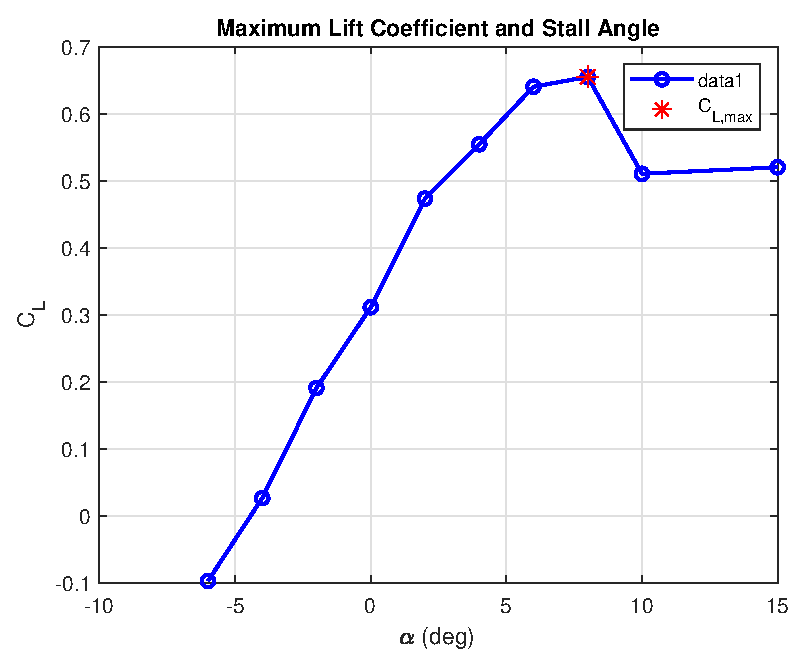
\includegraphics[width=0.6\textwidth]{CLmax_vs_alpha.eps}
    \caption{Maximum lift and stall angle}
    \label{fig:CLmax}
\end{figure}

\subsection{Lift Slope and Zero-Lift Angle}

Using a linear fit to the \( C_L \) vs. \( \alpha \) data in the pre-stall region (Figure~\ref{fig:CLfit}), the lift slope was determined to be:
\[
\frac{dC_L}{d\alpha} = 0.0634 \quad \text{(per deg)}, \quad \alpha_{L=0} = -4.72^\circ
\]

\begin{figure}[H]
    \centering
    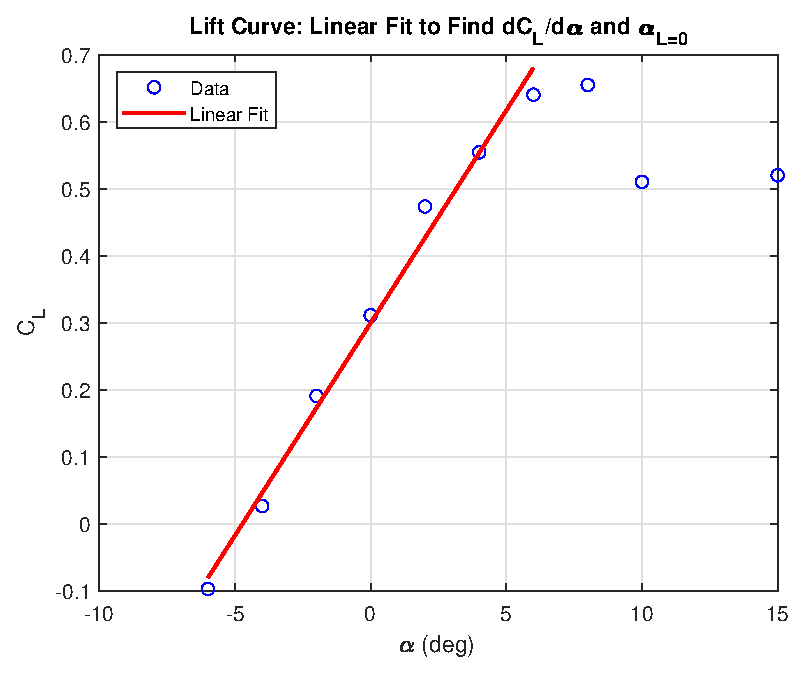
\includegraphics[width=0.6\textwidth]{CL_vs_alpha_linear_fit.eps}
    \caption{Linear fit of \( C_L \) vs. \( \alpha \) for lift slope and zero-lift angle}
    \label{fig:CLfit}
\end{figure}

\subsection{Pitching Moment vs. Angle of Attack}

The pitching moment coefficient \( C_M \) decreased linearly with \( \alpha \) for the tail-on configuration, with a slope of:
\[
\frac{dC_M}{d\alpha} = -0.0243 \quad \text{(tail-on)}, \quad \frac{dC_M}{d\alpha} = 0.0135 \quad \text{(tail-off)}
\]

The tail-off configuration showed a positive slope, indicating longitudinal instability. The results are shown in Figure~\ref{fig:CMtail}.

\begin{figure}[H]
    \centering
    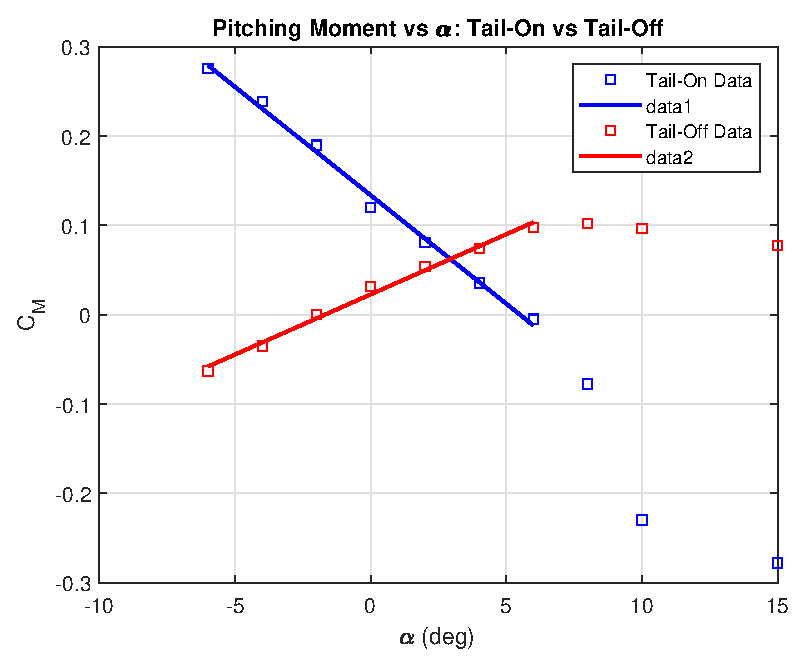
\includegraphics[width=0.6\textwidth]{CM_vs_alpha_tailon_tailoff.eps}
    \caption{Pitching moment coefficient vs. angle of attack (tail-on and tail-off)}
    \label{fig:CMtail}
\end{figure}

\subsection{Yawing Moment vs. Sideslip Angle}

Directional stability was evaluated by plotting \( C_N \) vs. sideslip angle \( \beta \). The tail-on configuration had a positive slope of \( \frac{dC_N}{d\beta} = 0.0019 \), confirming directional stability. The tail-off configuration showed a negative slope of \( \frac{dC_N}{d\beta} = -0.0009 \), indicating instability. Results are shown in Figure~\ref{fig:CNtail}.

\begin{figure}[H]
    \centering
    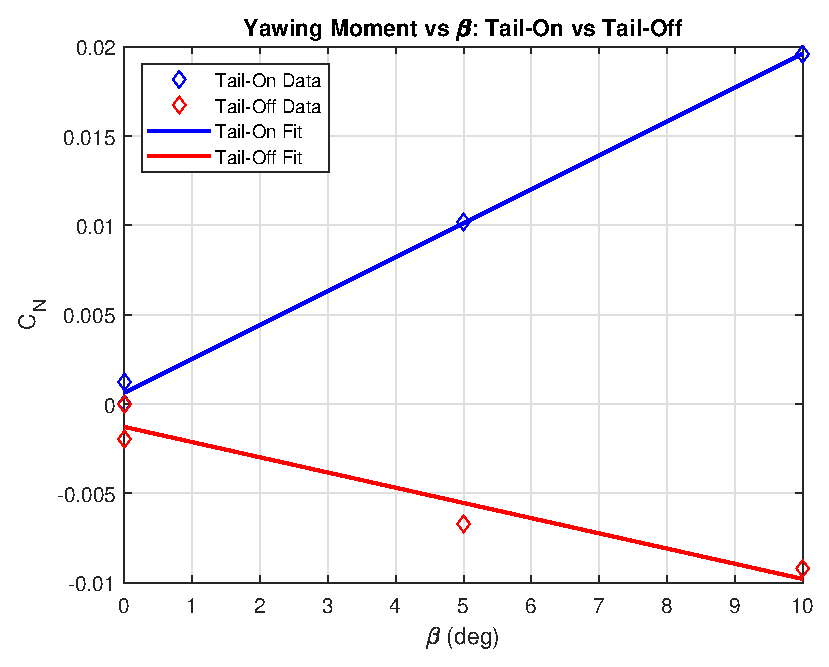
\includegraphics[width=0.6\textwidth]{CN_vs_beta_tailon_tailoff.eps}
    \caption{Yawing moment coefficient vs. sideslip angle (tail-on and tail-off)}
    \label{fig:CNtail}
\end{figure}

\subsection{Lift-to-Drag Ratio and Efficiency}

The lift-to-drag ratio \( C_L/C_D \) was computed for each data point. The maximum value was:
\[
\left( \frac{C_L}{C_D} \right)_{\max} = 16.214 \quad \text{at } \alpha = 4^\circ
\]

\begin{figure}[H]
    \centering
    \includegraphics[width=0.6\textwidth]{CL_over_CD_vs_alpha.eps}
    \caption{Lift-to-drag ratio vs. angle of attack}
    \label{fig:LD}
\end{figure}

\subsection{Drag Polar and Oswald Efficiency Factor}

The drag polar was fitted with the standard parabolic model:
\[
C_D = C_{D,0} + K C_L^2
\]
with fit results:
\[
C_{D,0} = -0.0100, \quad K = 0.4244
\]

Using the drag polar coefficient \( K \), the Oswald efficiency factor was computed as:
\[
e = \frac{1}{\pi K AR} = 0.0961
\]

The fit is shown in Figure~\ref{fig:DragPolar}.

\begin{figure}[H]
    \centering
    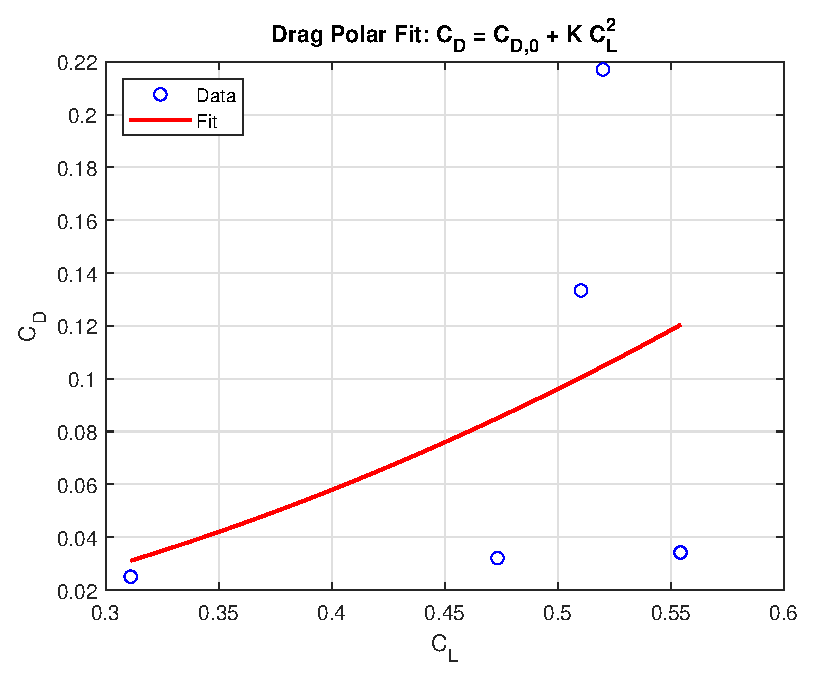
\includegraphics[width=0.6\textwidth]{DragPolarFit_CD_vs_CL.eps}
    \caption{Parabolic drag polar fit for Oswald efficiency factor}
    \label{fig:DragPolar}
\end{figure}

\subsection{Pitching and Yawing Moments (Single Configurations)}

Figures~\ref{fig:CMvsAlpha} and~\ref{fig:CNvsBeta} show the isolated tail-on behavior for moment coefficients:

\begin{figure}[H]
    \centering
    \includegraphics[width=0.6\textwidth]{CM_vs_alpha.eps}
    \caption{Pitching moment coefficient vs. angle of attack (tail-on)}
    \label{fig:CMvsAlpha}
\end{figure}

\begin{figure}[H]
    \centering
    \includegraphics[width=0.6\textwidth]{CN_vs_beta.eps}
    \caption{Yawing moment coefficient vs. sideslip angle (tail-on)}
    \label{fig:CNvsBeta}
\end{figure}

Each measured data point included a Root Mean Square Deviation (RMSD), which represents the standard deviation of balance readings over the measurement period. Although not directly propagated through the coefficient calculations, RMSD values offer insight into the reliability of the balance and highlight potential data anomalies at high angles of attack.

\subsection{Reynolds Number Estimate}

The Reynolds number (\(Re\)) for this experiment was calculated based on the mean aerodynamic chord length and estimated tunnel conditions. Since the dynamic pressure was maintained at a constant value, and no freestream velocity was explicitly measured, standard atmospheric assumptions were used to estimate flow properties. The Reynolds number is defined as:

\[
Re = \frac{\rho V c}{\mu}
\]

Where:
\begin{itemize}
    \item \(c = 0.456 \, \text{m}\) is the mean aerodynamic chord of the model
    \item \(V = 30 \, \text{m/s}\) is an estimated tunnel velocity based on subsonic testing standards
    \item \(\rho = 1.2041 \, \text{kg/m}^3\) is the density of air at 20°C and 1 atm
    \item \(\mu = 1.825 \times 10^{-5} \, \text{Pa}\cdot\text{s}\) is the dynamic viscosity of air at 20°C
\end{itemize}

Substituting the values:

\[
Re = \frac{(1.2041)(30)(0.456)}{1.825 \times 10^{-5}} = \boxed{9.03 \times 10^5}
\]

This Reynolds number indicates transitional flow near the upper end of the laminar range, which is typical for low-speed wind tunnel testing of small-scale aircraft models.


\section{Discussion}

To isolate the true aerodynamic forces and moments acting solely on the model, a two-level tare correction was applied. The first subtraction \([F_{\text{model on, wind on}} - F_{\text{model on, wind off}}]\) removed static forces due to the model weight and mount loading. The second subtraction \([F_{\text{model off, wind on}} - F_{\text{model off, wind off}}]\) eliminated wind-induced forces acting on the support structure. This methodology ensures that the final results represent the net aerodynamic forces and moments acting on the model alone.

The lift coefficient \(C_L\) increased linearly with angle of attack until stall occurred at approximately \(\alpha = 8^\circ\), with \(C_{L,\text{max}} = 0.6549\). This behavior is consistent with expectations from classical airfoil theory and published data on similar configurations~\cite{anderson2017fundamentals}. A linear fit to the pre-stall data gave a lift slope of \(\frac{dC_L}{d\alpha} = 0.0634\) per degree, and the zero-lift angle of attack was found to be \(\alpha_{L=0} = -4.72^\circ\). These values are within acceptable bounds for moderate aspect ratio wings tested in low-speed wind tunnels~\cite{rae1984low}.

The drag polar, fitted with a parabolic model, yielded \(C_{D,0} = -0.0100\) and \(K = 0.4244\). While a negative zero-lift drag coefficient is physically unrealistic, it is likely the result of minor inconsistencies in tare subtraction or force measurement noise. This also contributed to an unusually low Oswald efficiency factor of \(e = 0.0961\), significantly below the typical range of 0.7–0.9 for similar configurations~\cite{anderson2017fundamentals}. These anomalies suggest that the RMS deviations in some force components (particularly \(F_x\)) may have impacted the drag curve fit more than the lift-based analyses.

The aircraft's longitudinal stability was assessed by evaluating the slope \(\frac{dC_M}{d\alpha}\) for both configurations. In the tail-on case, the slope was negative (\(-0.0243\)), indicating longitudinal static stability as expected. Conversely, the tail-off configuration produced a positive slope (\(+0.0135\)), confirming longitudinal instability and demonstrating the crucial role of the horizontal stabilizer.

Directional stability was analyzed using the slope \(\frac{dC_N}{d\beta}\). With the tail on, the slope was positive (\(+0.0019\)), confirming that the vertical tail provided a restoring yawing moment in response to sideslip. Without the tail, the slope reversed to negative (\(-0.0009\)), showing directional instability. These findings directly support classical stability theory and confirm the effectiveness of the tail surfaces in maintaining directional and longitudinal equilibrium~\cite{anderson2017fundamentals}.

Ambient conditions such as \(T_{\text{amb}}\) and \(P_{\text{amb}}\) were recorded and found to be stable across test configurations. However, they were not used in coefficient calculations due to the use of calibrated tunnel dynamic pressure \(q\). The RMS deviations were recorded for all runs and suggest that some components, particularly yawing and pitching moments, showed higher uncertainty during tail-off measurements, possibly due to reduced aerodynamic damping or slight misalignments.

Some observed variability in the data—especially in force and moment readings at higher angles of attack—may be attributed to wind tunnel turbulence and model mounting inconsistencies. Although the SDSU low-speed wind tunnel maintains a relatively low turbulence intensity (turbulence factor of 1.27), fluctuations in freestream conditions can still affect sensitive measurements such as drag and yawing moments. Additionally, minor misalignments or compliance in the mounting hardware can introduce asymmetries, particularly when tail-off configurations reduce the restoring effects of aerodynamic surfaces. These factors could contribute to the slightly noisy behavior seen in the \( C_N \) and \( C_M \) curves and to the drag polar's negative \( C_{D,0} \) offset.

\section{Conclusion}

This experiment successfully demonstrated how aerodynamic forces and moments can be isolated and analyzed for a full aircraft model in a subsonic wind tunnel. By applying two levels of tare correction, the net aerodynamic loads were extracted, enabling accurate calculation of lift, drag, and moment coefficients.

The lift curve slope and stall behavior were consistent with theoretical expectations. The pre-stall region exhibited a linear \( C_L \) vs. \( \alpha \) relationship with a reasonable slope, and stall occurred near \( \alpha = 8^\circ \), aligning with airfoil theory. The tail-on configuration produced negative \(\frac{dC_M}{d\alpha}\) and positive \(\frac{dC_N}{d\beta}\), confirming longitudinal and directional stability. Conversely, the tail-off configuration exhibited a reversal in both slopes, confirming the stabilizing roles of the horizontal and vertical tails. These trends aligned with classical aerodynamic stability theory~\cite{anderson2017fundamentals, kuethe1986foundations}.

One surprising result was the appearance of a slightly negative zero-lift drag coefficient in the fitted drag polar, along with a notably low Oswald efficiency factor. These anomalies may reflect imprecision in streamwise force measurements, balance noise, or residual tare asymmetries—particularly in the tail-off configurations.

To refine the experimental process in future implementations, the following improvements are recommended:
\begin{itemize}
    \item Increase data averaging or sampling frequency to reduce RMSD-induced noise.
    \item Implement error bars on coefficient plots using the RMSD values as a basis for uncertainty estimation.
    \item Rigorously verify model alignment and fixture repeatability between runs.
    \item Incorporate ambient conditions into Reynolds number or density-based pressure calculations.
\end{itemize}

Overall, the experiment reinforced theoretical aerodynamic principles, illustrated the stabilizing effects of tail surfaces, and highlighted practical challenges in wind tunnel testing, including tare removal accuracy and sensitivity to mounting precision.

\section*{Acknowledgments}
The author would like to thank Dr. Xiaofeng Liu for his guidance and Teacher's Assistant Andrew Balolong for assistance during the experiment.

\bibliography{references}
\bibliographystyle{new-aiaa}

\section{Appendix}
\appendix

\section{Derivation of Tare Correction Equation}
\label{sec:appendix-tare}

To isolate the true aerodynamic forces and moments acting on a wind tunnel model, we apply a two-level tare correction based on the principle of superposition. The measured signals from the force balance include contributions from both aerodynamic loading and structural artifacts such as model weight and support interactions.

Let the measured force vector be denoted as:
\[
\mathbf{F}_{\text{meas}} = \mathbf{F}_{\text{aero}} + \mathbf{F}_{\text{tare}}
\]
where:
\begin{itemize}
    \item \( \mathbf{F}_{\text{aero}} \) is the true aerodynamic force (the quantity of interest),
    \item \( \mathbf{F}_{\text{tare}} \) includes model weight, mount-induced strain, and wind-induced forces on the support structure.
\end{itemize}

The tare correction is derived by executing four configurations:
\begin{enumerate}
    \item Model \textbf{on}, Wind \textbf{on}: \( \mathbf{F}_{1} = \mathbf{F}_{\text{aero}} + \mathbf{F}_{\text{tare, model}} + \mathbf{F}_{\text{tare, support}} \)
    \item Model \textbf{on}, Wind \textbf{off}: \( \mathbf{F}_{2} = \mathbf{F}_{\text{tare, model}} \)
    \item Model \textbf{off}, Wind \textbf{on}: \( \mathbf{F}_{3} = \mathbf{F}_{\text{tare, support}} \)
    \item Model \textbf{off}, Wind \textbf{off}: \( \mathbf{F}_{4} = \mathbf{0} \)
\end{enumerate}

The tare-corrected aerodynamic force is thus:
\[
\mathbf{F}_{\text{aero}} = (\mathbf{F}_{1} - \mathbf{F}_{2}) - (\mathbf{F}_{3} - \mathbf{F}_{4})
\]

This simplifies to:
\[
\mathbf{F}_{\text{aero}} = [\mathbf{F}_{\text{model on, wind on}} - \mathbf{F}_{\text{model on, wind off}}] - [\mathbf{F}_{\text{model off, wind on}} - \mathbf{F}_{\text{model off, wind off}}]
\]

\textbf{Assumptions:}
\begin{itemize}
    \item The balance responds linearly to force inputs.
    \item Mounting effects are repeatable and subtractable.
    \item Environmental conditions (like pressure and temperature) remain constant across tare runs.
\end{itemize}

\textbf{Theoretical Basis:} This correction aligns with the superposition principles described in classical potential flow theory. As shown in Chapter 6 of Anderson~\cite{anderson2017fundamentals}, force and potential contributions from multiple sources (e.g., point sources, doublets, and freestream) are additive. For instance, the surface velocity on a sphere from a uniform freestream and a doublet is:
\[
V_\theta = \frac{3}{2}V_\infty \sin \theta
\]
and the pressure coefficient is:
\[
C_p = 1 - \frac{9}{4}\sin^2 \theta
\]

Similarly, in wind tunnel testing, we isolate the contribution from the aerodynamic "freestream" effect by subtracting off the influences from support and mount “sources.”

\textbf{Conclusion:} This tare correction enables precise recovery of aerodynamic coefficients from complex, superimposed measurements. The corrected forces were subsequently converted into non-dimensional coefficients using:
\[
C_L = \frac{F_z}{qS}, \quad C_D = \frac{F_x}{qS}, \quad C_M = \frac{M_y}{qSc}, \quad C_N = \frac{M_z}{qSb}
\]
as documented in the Results section.


\section{Original Experimental Data}
\label{sec:appendix}

The original wind tunnel force and moment measurements, as well as Root Mean Square Deviation (RMSD) values, are shown in the figures below for each run configuration.

\begin{figure}[H]
    \centering
    \includegraphics[width=0.95\textwidth]{run_data_page1.png}
    \caption{Raw data for Run 1–5 (model on/off, wind on/off)}
    \label{fig:rawdata1}
\end{figure}

\begin{figure}[H]
    \centering
    \includegraphics[width=0.4\textwidth]{rmsd_page2.png}
    \caption{Root Mean Square Deviation (RMSD) data for all runs}
    \label{fig:rmsd}
\end{figure}

\section{MATLAB}
The following MATLAB script \cite{matlab} was used for all Data Reduction and Graph Plotting:
\lstinputlisting[language=Matlab, caption={MATLAB Code for Data Analysis}]{AE303_Lab5.m}

\end{document}